\chapter{Methodology}\label{chapter:methodology}
In this chapter, the simulator used to investigate the research questions is described. An overview of the system is presented in section \ref{section:systemt architecture}. Section \ref{section:genetic algorithm} includes implementation details, and design decisions made when implementing the genetic algorithm which is the foundation for all the population distributed genetic algorithms. Sections \ref{section:population distributed gas implementation details} contain implementation details of the population distributed genetic algorithms. The wind scenarios used to evaluate the different population distributed genetic algorithm are described in section \ref{section:scenarios}, and the choice of implementing the genetic algorithm from scratch is defended in section \ref{section:motivation}.


\section{System Architecture}\label{section:systemt architecture}
The program is implemented in Java and the interactions between the different classes of the program are shown in figure \ref{figure:class diagram}. The GeneticAlgorithm class is extended by the three population distributed genetic algorithm classes: IslandModel, CellularModel and PoolModel. In addition, the GeneticAlgorithm class is also implemented as instances in all three population distributed algorithms. The main loop of the program is contained in the GeneticAlgorithm class. It uses instances of the classes WindScenario, WindFarmLayoutEvaluator, Population, AdultSelection, ParentSelection, Crossover and Mutation. AdultSelection and ParentSelection are interfaces that needs to be implemented if new methods are to be added to the program, and Crossover is an abstract class containing one method which every Crossover class must implement. Mutation is a class containing four different mutation methods. 


\begin{figure}[h!]
\begin{center}
\includegraphics[scale=0.35]{images/"Class Diagram"}
\caption{Class Diagram.}
\label{figure:class diagram}
\end{center}
\end{figure}


\section{Genetic Algorithm: Implementation Details}\label{section:genetic algorithm}
As mentioned in chapter \ref{chapter:background}, the genetic algorithm is a four step process: Adult selection, parent selection, recombination such as crossover and mutation, and fitness evaluation as shown in figure \ref{figure:genetic algorithm steps}. Implementation details of each step is described in the subsequent sub sections. In addition, the wind-, wake-, and power model used in evaluating the genetic algorithm are described in the following subsections since these are crucial to understanding the fitness function. 


\begin{figure}[h!]
\begin{center}
\includegraphics[scale=0.3]{images/"genetic algorithm"}
\caption{Genetic algorithm.}
\label{figure:genetic algorithm steps}
\end{center}
\end{figure}


\noindent The simple genetic algorithm is implemented using the Master/Slave model. The Master/Slave model is the most common way of implementing a simple genetic algorithm. Evaluation of the different layouts in a population is by far the most time consuming step of the genetic algorithm. The Master/Slave model copes with this problem by distributing the evaluation to different slave processes, one for each core of the computer. By evaluation the population in parallel, the heaviest computational load is split between all the cores of the computer and the speed-up is proportional to the number of cores. The Master/Slave model is displayed in figure \ref{Master-Slave Model}.\\


\begin{figure}[h!]
\begin{center}
\includegraphics[scale=0.3]{images/"population distributed genetic algorithms"/"master-slave model"}
\caption{Master-slave model. The master process distributes the population to different slave processes, which calculate the fitness of each individual and return the results to the master process \citep{Gong}.}
\label{Master-Slave Model}
\end{center}
\end{figure}


\subsection{Representation}
As in most of the studies presented in chapter \ref{chapter:relatedwork}, the individuals implemented for the genetic algorithm for this thesis are represented by binary strings. However, each position in the binary string can be directly mapped to a position in the terrain kept in an array called ''grid''. The purpose behind this design decision is that not all positions in the terrain, when dividing the terrain into a squared grid, are legal turbine positions because of the existence of obstacles. By implementing individuals this way, the genetic operations can be performed on individuals without having to check for illegal positions since this is already taken care of as soon as the scenario is read from file. Also, this design decision makes sure that no space is wasted keeping illegal positions in the binary representation. Figure \ref{figure:representation} shows how a given terrain is represented using a binary string and the grid-array. The grid to the left in the figure represents the terrain. Red cells represent illegal positions while grey cells represents legal positions. An individual and the grid array are presented to the right. Since there are only 9 legal positions in the terrain the individual has length 9. The grid-array contains the (x,y)-positions of each legal positions in the terrain. The given individual has the value 1 in positions 2, 4 and 8 respectively (zero indexed), meaning that wind turbines are positioned in the (x,y)-positions in positions 2, 4 and 8 in the grid-array, meaning position (1,2), (2,0) and (3,2) in the terrain. Wind parameters and obstacle positions are read into the program from the scenarios provided by GECCO 2016, these will be described later in this chapter.


\begin{figure}[h!]
\begin{center}
\includegraphics[scale=0.5]{images/"representation program"}
\caption{Individual representation. The grey squares represent legal turbine positions in the terrain, while the red represent illegal positions. Since there are only nine legal positions in this example, an individual is represented as a binary string of length 9. The grid array is shared between all the individuals and holds the (x, y)-coordinates for each legal position.}
\label{figure:representation}
\end{center}
\end{figure}


\subsection{Adult Selection}\label{subsection:adult selection}
Adult selection is the process of selecting which individuals that are allowed to step into the adult pool and thereby become potential parents for the next generation of individuals. Three adult selection mechanisms were implemented in this thesis: Full generational replacement,  generational mixing, and overproduction. Each method was tested in order to decide which adult selection method was more suitable for solving the wind farm layout optimization problem. \\

\noindent Full generational replacement, the simplest adult selection mechanism, replaces the previous adult population with the newly generated child population. The second method, generational mixing, is illustrated in figure \ref{figure:generational mixing}. As the name suggests, generational mixing mix the previous adult pool together with the new child pool and selects the best individuals from the mix to become the new adult population. As can be seen in the figure, the new adult pool consists of the best individuals from both the newly generated child pool and the previous adult pool. The two individuals with fitness 2 and 3 are selected from the child pool, and the two individuals with fitness 4 and 4 is selected from the previous adult pool. The new child population will therefore contain individuals with fitness 4, 2, 3 and 4, instead of fitness of 5, 6, 3 and 2, which would be the adult population if full generational replacement was used. 


\begin{figure}[h!]
\begin{center}
\includegraphics[scale=0.2]{images/"adult selection"/"generational mixing"}
\caption{Generational mixing. The best individuals, from the pool consisting of individuals from the previous adult population and the new child population are selected as new the adult population.}
\label{figure:generational mixing}
\end{center}
\end{figure}


\noindent Overproduction, the third adult selection mechanism, is illustrated in figure \ref{figure:overproduction}. The newly generated child population consist of twice as many individuals as there are room for in the adult population. Therefore, the children have to compete against each other for the spots in the adult pool. \\


\begin{figure}[h!]
\begin{center}
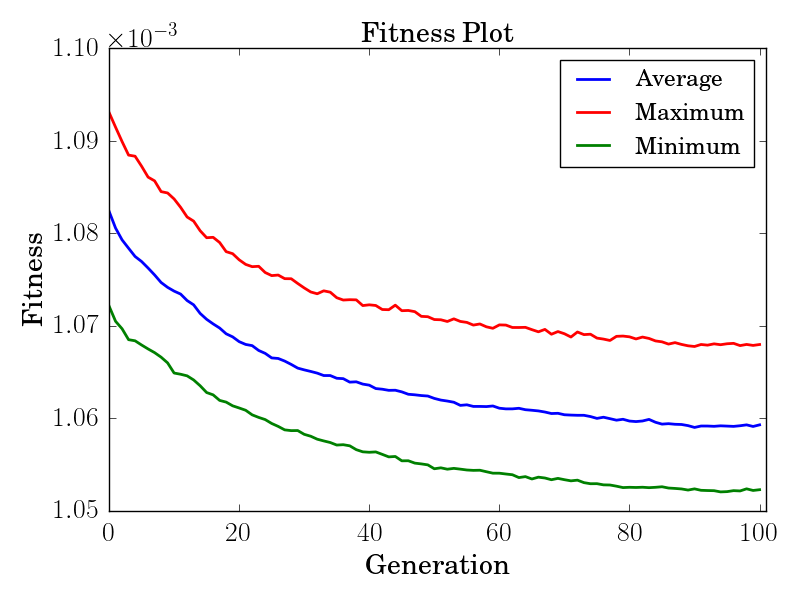
\includegraphics[scale=0.2]{images/"adult selection"/overproduction}
\caption{Overproduction. The newly generated child population consist of twice as many individuals as there are room for in the adult population. Therefore, only the fittest individuals from the large child population grow up into adults.}
\label{figure:overproduction}
\end{center}
\end{figure}



\subsection{Parent Selection}\label{subsection:parent selection}
Parent selection is the process of deciding which adults become parents for the next child generation. When choosing parent selection method there are a few concerns that needs to be addressed. First, it is important that parents with good genes, i.e. lower fitness, gets their genes transferred to the next generation. However, it is also important to keep diversity in the population so that one does not end up with a sub-optimal solution; a local maximum. Two parent selection methods are implemented for the genetic algorithm for this thesis: Tournament selection and roulette wheel selection. \\

\noindent In tournament selection, a given number of individuals are drawn randomly from the population. The number of individuals drawn is decided by the variable \textit{tournament size}. These individuals compete in a tournament for one spot in the parent pool. The individual with best fitness is  selected as a parent. These tournaments continue until the adult pool is full. Figure \ref{figure:tournament selection} shows how tournament selection works. As can be seen in the figure, three individuals are drawn randomly from the adult pool, meaning that the tournament size in this example is 3. The best individual, the individual with fitness 4 is the tournament winner and is allowed to enter the adult pool. In order to maintain diversity in the population there is a small probability that parents are selected randomly from the adult pool instead of with tournament selection. This probability is called \textit{epsilon} and makes sure that a small percent of the parents that might not currently be best are not killed of right away. Different values of the \textit{tournament size} variable needs to be tested in order to find the settings that allow the algorithm to explore different solutions, but that also prioritize the best solutions. In chapter \ref{chapter:results}, results obtained for different values of \textit{tournament size} and \textit{epsilon} are compared. \\


\begin{figure}[h!]
\begin{center}
\includegraphics[scale=0.2]{images/"parent selection"/"tournament selection"}
\caption{Tournament selection. Three individuals with fitness 9, 4 and 6 respectively, are selected randomly from the adult population. The individuals with best fitness, fitness 4, is the tournament winner and is selected into the parent pool.}
\label{figure:tournament selection}
\end{center}
\end{figure}


\noindent Roulette wheel selection assigns a probability of being chosen as parent to each individual proportional to its fitness. Individuals with better fitness will therefore have a higher probability of beings selected into the parent pool. Figure \ref{figure:roulette wheel selection} shows how roulette wheel selection works. The roulette wheel on the left shows the probability for each of the four individuals being selected. Since individual$_4$ has the best fitness, it has a larger probability of being selected than the others. \\


\begin{figure}[h!]
\begin{center}
\includegraphics[scale=0.5]{images/"parent selection"/"roulette wheel selection"}
\caption{Roulette wheel selection. The roulette wheel is shown to the left, the four individuals to the right. Individual$_4$ has a four times better fitness than individual$_2$ and therefore has a four times larger probability of being selected.}
\label{figure:roulette wheel selection}
\end{center}
\end{figure}


\subsection{Genetic Operations}\label{subsection:genetic operations}
This subsection gives an overview over the genetic operations used to produce the next child generation. Three crossover methods, elitism and four mutation methods are implemented and will be presented. 


\subsubsection{Crossover and Elitism}
Crossover is the recombination method utilized by the genetic algorithm to perform sexual reproduction. A crossover operation produced two children by recombining genes of two parent individuals. The genetic algorithm implemented for this thesis has three crossover methods to chose from: Single point crossover, two point crossover and uniform crossover \citep{Magalhaes-Mendes}. These are all presented in figure \ref{figure:crossover methods}. As shown in figure \ref{figure:single point crossover}, single point crossover uses randomly generated position, called the crossover point, to perform recombination. All genes from the first parent prior to the crossover point are copied to the first child, and all genes after the crossover point are copied to the second child, and all genes from the second parent prior to the crossover point is copied to the second child, and all genes after the crossover point is copied to the first child. Two point crossover is similar to single point crossover, except that it uses two crossover points instead of one. This is shown in figure \ref{figure:two point crossover}. In uniform crossover, there is a fifty percent probability that each gene will be drawn from each parent as shown in figure \ref{figure:uniform crossover}. This crossover method mix up the parent genes more than the two others, therefore more gene patterns will be lost using this method. Even though crossover is the main recombination method it is not used for creating every child individual. Some child individuals are copies of their parents with potential small mutation in their genes. The number of individuals created using crossover is decided by the crossover rate. Crossover rates are usually kept pretty high since the goal is to evolve new and better solutions, however test runs presented in chapter \ref{chapter:results} do confirm that it is good to let a percentage of the children be produced without crossover. \\


\begin{figure}[h!]
    \centering
    \begin{subfigure}[b]{0.3\textwidth}
        \includegraphics[width=\textwidth]{images/crossover/"Single point crossover"}
        \caption{}
        \label{figure:single point crossover}
    \end{subfigure}
    ~ 
    \begin{subfigure}[b]{0.3\textwidth}
        \includegraphics[width=\textwidth]{images/crossover/"Two point crossover"}
        \caption{}
        \label{figure:two point crossover}
    \end{subfigure}
    ~
    \begin{subfigure}[b]{0.3\textwidth}
        \includegraphics[width=\textwidth]{images/crossover/"Uniform crossover"}
        \caption{}
        \label{figure:uniform crossover}
    \end{subfigure}
    \caption{Crossover methods: (a) Single point crossover, (b) two point crossover, and (c) uniform crossover.}
    \label{figure:crossover methods}
\end{figure}


\noindent A method used to make sure that the best individuals in the population does not get killed of by accident is called \textit{elitism}. Elitism simply takes the best individual(s) from the parent population and copies it(them) directly into the new child population without performing any genetic operations on it(them). Elitism is commonly used with genetic algorithm and will be used in this thesis. 


\subsubsection{Mutation}
Although crossover is a powerful genetic operator that makes sure that child individuals inherit genes from the best parent individuals, it is not enough by itself. Without any way to mutate genes, one can end up with a population where every individual has the same gene value in the same position, this means that no recombination method will be able to change the value of that gene. Mutation is the operation used by the genetic algorithm to make sure that the population do not get sterile. In nature, genes can be mutated in numerous ways. In this thesis, three mutation methods are implemented to mimic the mutation methods that can happen in genes \citep{Soni}, these are called: Flip mutation, interchanging mutation, and inversion mutation. Flip mutation, shown in figure \ref{figure:flip mutation}, is the most common mutation method used in genetic algorithms. As it's name implies, flip mutation works by flipping the value of bits in the genotype. Usually, mutation rates are low since one do not want mutation to make to many changes to the good genes inherited from parent individuals, but simply introduce some diversity. Therefore, only a couple of bits are mutated in each genotype each generation. Interchange mutation and inversion mutation are rarely used in genetic algorithms, however they are included in this thesis to introduce even more diversity in the population and hopefully help the genetic search finding even better solutions. They both introduce more change than flip mutation, and will be assigned rates even lower than the mutation rate for flip mutation. Figure \ref{figure:interchange mutation} and \ref{figure:inversion mutation} shows interchange- and inversion mutation respectively. Interchange mutation works by picking two random genes and interchange their values, while inversion mutation works by picking two random positions and invert each gene between those positions. 


\begin{figure}[h!]
    \centering
    \begin{subfigure}[b]{0.3\textwidth}
        \includegraphics[width=\textwidth]{images/mutation/"flip mutation"}
        \caption{}
        \label{figure:flip mutation}
    \end{subfigure}
    ~ 
    \begin{subfigure}[b]{0.3\textwidth}
        \includegraphics[width=\textwidth]{images/mutation/"interchanging mutation"}
        \caption{}
        \label{figure:interchange mutation}
    \end{subfigure}
    ~
    \begin{subfigure}[b]{0.3\textwidth}
        \includegraphics[width=\textwidth]{images/mutation/"inversion mutation"}
        \caption{}
        \label{figure:inversion mutation}
    \end{subfigure}
    \caption{Mutation methods: (a) Single point crossover, (b) two point crossover, and (c) uniform crossover.}
    \label{figure:mutation methods}
\end{figure}


\subsection{Wind-, Wake- and Power Model}\label{subsection:wind-, wake- and power model}
The evaluation class uses the same wake-, wind- and power model as \cite{Kusiak}. The wake model used is the classical Jensen model \citep{Jensen}, which is used in almost every study of the wind farm layout optimization problem, as can be seen in table \ref{table:overview related work}. \\

\noindent Wind distribution is modeled using the Weibull distribution, a continuous probability distribution shown to model wind distribution quite well \citep{Justus}. The probability density function is shown in equation \ref{equation:Weibull}


\begin{equation}
f(x; c, k)  = 
\begin{cases}
\frac{k}{c} \left( \frac{x}{c} \right)^{k-1} e^{- \left( \frac{x}{c} \right)^k } & \text{if} \hspace{1mm} x \geq 0 \\
0                                                                                                                      & \text{if} \hspace{1mm}     x < 0
\end{cases}
\label{equation:Weibull}
\end{equation}


\noindent where $k$ is called the shape parameter and $c$ is the scale parameter, and $k, c > 0$. In most of the wind scenarios provided by GECCO 2016, $k \approx 2$, this is shown empirically to be a good value for wind speed distribution \citep{Justus}. On the other hand, the shape parameter vary for each wind direction. Figure \ref{figure:weibull distribution} shows the Weibull distribution plotted for $k = 2$ and for different values of $c$. \\


\begin{figure}[h!]
\begin{center}
\includegraphics[scale=0.4]{images/"Weibull"}
\caption{The Weibull distribution plotted for $k = 2$ for different values of the scale parameter $c$.}
\label{figure:weibull distribution}
\end{center}
\end{figure}

\noindent The wind scenarios used in this thesis are therefore a specification of the shape- and scale parameters for every wind direction, where wind direction is partitioned into 24 different directions. Twenty wind scenarios are provided by GECCO 2016, 10 which simply specify wind distribution parameters, and 10 that specify wind distribution parameters and locations of obstacles. \\

\noindent The power curve used is also the same as used in \cite{Kusiak}, it is the linear function shown in equation \ref{equation:Power Curv (API)},

\begin{equation}
 f(v) = 
  \begin{cases} 
   0                                  & \text{if }     v < v_{cut-in} \\
   \lambda v + \eta           & \text{if }     v_{cut-in} \leq v \leq v_{rated} \\
   P_{rated}                        & \text{if }     v_{cut-out} > v > v_{rated}. \\
  \end{cases}
  \label{equation:Power Curv (API)}
\end{equation}

\noindent Here $\lambda$ is the slope parameter, $v$ the wind speed, $\eta$ the intercept parameter, $P_{rated}$ is the fixed power output, and $v_{cut-in}$ is the cut-in speed; the minimum speed for which the turbine produces power, and $v_{cut-out}$ is the cut-out speed; the maximum wind speed for which the turbine is kept on. 


\subsection{Fitness Function}\label{subsection:fitness function}
The main task of the evaluation classes is to calculate the fitness of each individual based on the fitness function.  The fitness function to be minimized is provided by GECCO 2016, and is displayed in equation \ref{Objective function}.\\

\begin{small}
\begin{equation}
fitness =  \frac{ \left( c_t \cdot n + c_s \cdot \floor*{\frac{n}{m}} \right) \left( \frac{2}{3} + \frac{1}{3} \cdot e^{-0.00174n^2} \right) + c_{OM} \cdot n}{\left( \frac{1 - (1 + r)^{-y}}{r} \right) } \cdot \frac{1}{8760 \cdot P} + \frac{0.1}{n}
\label{Objective function} 
\end{equation}
\end{small}


\noindent Description and numerical values of all parameters given in equation \ref{Objective function} are displayed in table \ref{Parameters}. As can be seen in this table, the values of $n$, the number of turbines, and $P$, farm energy output, are not given. This is because the number of turbines, together with the turbine positions, are the parameters to be optimized by the genetic algorithm. Farm energy output is the indirect parameter that we are trying to optimize. It is dependent on turbines count, position, wind scenario and so on, and is of course therefore not provided in table \ref{Parameters} either.\\


\begin{table}[h!]
\begin{center}
\caption{Description and value of each parameter used in the objective function provided by GECCO 2015.}
\label{Parameters}
\begin{tabular}{l|l|l}
\textbf{Parameter} & \textbf{Description} & \textbf{Value} \\ 
\hline 
$c_t$ & Turbine cost (usd) & 750 000 \\ 
$c_s$ & Substation cost (usd) & 8 000 000 \\ 
$m$ & Turbines per substation & 30 \\ 
$r$ & Interest rate & 0.03 \\ 
$y$ & Farm lifetime (years) & 20 \\ 
$c_{OM}$ & Yearly operating costs per turbine & 20 000 \\ 
$n$ & Number of turbines &  \\ 
$m$ & Farm energy output &  \\  
\end{tabular} 
\end{center}
\end{table}


\noindent Intuitively, the objective function can be divided into different parts. The first parenthesis in the nominator of the first fraction is the construction cost, while the second parenthesis is the economies of scale and the third part of the nominator is yearly operating costs. The denominator represents the interests. The denominator of the second fraction describes yearly power output, while the number $0.1$ in the nominator of the last fraction is a farm size coefficient. \\


\section{Scenarios}\label{section:scenarios}


\begin{figure}[h!]
\begin{center}
\includegraphics[scale=0.4]{images/obstacles}
\caption{Obstacles are described in the scenarios with its (x, y)-boundaries.}
\label{figure:obstacles}
\end{center}
\end{figure}


GECCO 2016 has provided the contestants with 20 different wind scenarios for which the genetic algorithm can be tested on. Each wind scenario contain shape and scale parameters, k and c respectively, for each wind directions where wind direction is partitioned into slots that cover an 15 degree angle each, so that there are 24 different wind directions. Unavailable areas are described in the scenario by the parameters \textit{x$_{min}$, x$_{max}$, y$_{min}$} and \textit{y$_{max}$} as shown in figure \ref{figure:obstacles}. In the figure, two obstacles are described giving their (x, y)-boundaries. The boundaries of the obstacles are marked with black lines. The yellow area in the middle of the lines are the illegal areas. Each wind scenario also contain values for the constants ''width'', ''height'', ''number of turbines'' and ''wake free energy''. The scenarios are read from file at the beginning of each run of the genetic algorithm. 


\section{Population Distributed Genetic Algorithms: Implementation Details}\label{section:population distributed gas implementation details}


Now that the reader is familiar with how individuals are represented, which selection mechanisms and genetic operators that are implemented, how fitness is calculated, and how the scenarios look, it is time to go into details of how the population distributed genetic algorithms are implemented. Although the population distributed genetic algorithms were introduced in chapter \ref{chapter:background}, the details of how each step in figure \ref{figure:genetic algorithm steps} are implemented for each model was not given. Therefore, this section contains a detailed description of how the population distributed genetic algorithms are implemented. \\


\noindent One decision that can be mentioned here, because it applies to all the models below, is whether the three population distributed genetic algorithms are heterogeneous or homogeneous. In an homogeneous environment, the same rules apply to the entire model. This means that the same adult- and parent selection mechanisms, the same genetic operators and the same fitness function is used for the entire model, it is not different for different Islands (Island model), threads (Pool model) or areas (Cellular model). Even thought it would be very interesting to implement heterogeneous models, it is not done in this thesis. The reason behind this decision is that it is best to let the same rules apply to every part of every model when different models are compared.\\


\subsection{The Island Model}


\noindent The Island model works as follows: A population of individuals are partitioned into sub populations which are distributed onto different Islands. An Island can be connected to one or more Islands and individuals on one Island can migrate to other Islands following one of the migration routes. Table \ref{table:parameter description island model} gives an description of the Island model parameters. For a number of generations, decided by the variable \textit{migration interval}, the population on one Island follow the steps of the simple genetic algorithm from figure \ref{figure:genetic algorithm steps}. However, when the population has evolved for \textit{migration interval} generations some individuals from one Island can migrate to another Island. These two steps continue until the total number of generations reaches some predefined value.\\


\noindent As mentioned in chapter \ref{chapter:background} the Island model can be implemented with either synchronized or asynchronized migration. Synchronized migration means that migration is performed at the same generation for all Island, and asynchronized migration means that migration can be performed whenever an Island is ready. In this thesis, the Island model is implemented with synchronous migration in order to not over-complicate the migration function.\\


\begin{table}[h!]
    \centering
    \caption{Island model parameter description.}
    \label{table:parameter description island model}
        \begin{tabular}{l|l}
         \textbf{Parameter} & \textbf{Description}  \\
         \hline
         Deme size  & Number of individuals on each Island (deme) \\
         Deme count & Number of Islands (demes) \\
         Migration rate & Number of individuals that migrate \\
         Migration interval & Number of generations between migration. \\
         Number of migrations & Total number of times migration is performed. \\
         Topology & Circular
    \end{tabular}
\end{table}


\noindent As mentioned, migration means that individuals migrates to another Island. In this thesis, migration from one Island to another means that the best individuals in Island \textit{i} is copied onto Island \textit{j} to replace the individuals with lowest fitness on Island \textit{j}. In other words, migration does not mean that the best individuals in Island \textit{i} leaves that Island, but that copies of them replace the individuals with worst fitness on Island \textit{j}. The number of individuals that migrate is decided by the parameter \textit{migration rate}.\\


\noindent As described in table \ref{table:parameter description island model} the topology implemented in this thesis is circular. This can be seen in figure \ref{figure:topology island model} where the legal migration routes are indicated by arrows. Since individuals are only allowed to migration in one direction with this topology it will take time (many generations) for the individual on the upper-right Island to travel to the upper-left Island since they have to go through both Islands on the bottom. This means that different parts of the solution space can be explored on different Island before individuals from one Island take over the entire population.


\begin{figure}
    \begin{center}
        \includegraphics[scale=0.5]{"island model topology"}
        \caption{Island model topology.}
        \label{figure:topology island model}
    \end{center}
\end{figure}


\subsection{Pool Model}


\noindent In the Pool model, the individuals are distributed in a resource pool. The resource pool is partitioned into equal size partitions so that one thread is responsible for one partition. Each thread selects \textit{x} individuals from the entire population, where \textit{x} is equal to the total population size divided by the total number of threads. Next, each thread generates a child pool by performing genetic operations on the selected individuals. After the new child pool is generated, each child individual is compared against the individual in the resource pool currently occupying its designated position. If the fitness of the new individuals is better than the fitness of the old individual the new child individual overwrites the old individuals. This is illustrated in figure \ref{figure:pool model update function}. As can be seen in the figure thread \textit{i} overwrites the individuals in positions 1, 3 and 4 in the partition it is responsible for.\\


\begin{figure}[h!]
\begin{center}
\includegraphics[scale=0.5]{images/"pool model update function"}
\caption{Pool model updating function. For each generation, each thread updates its region if the new individuals are better than the individuals currently occupying the position.}
\label{figure:pool model update function}
\end{center}
\end{figure}


\noindent The pool model is asynchronous by nature. The threads operate unaware of each other. Since each thread only writes to its own positions in the resource pool, it is not a problem that the threads work independently without any form of synchronization. By implementing the Pool model this way some parts of the resource pool might have better fitness that others because they have evolved for more generations than other parts. This property ensures that different parts of the search space is explored in different regions of the resource pool. \\


\noindent As mentioned above, parent individuals are selected from the entire resource pool. However, parents are not picked completely at random. For each parent selected a group of potential parents are selected at random from the resource pool, and these individuals compete for the spot in the parent pool by tournament selection. This guides the evolution in the right direction. Picking individuals at random might also work for this model since the new individuals are only written back if they are better than the previous individuals, however, this would make evolution extremely slow, and it would not make sense from an evolutionary point of view because the fittest individuals are not prioritized.


\subsection{Cellular Model}


\noindent The Cellular model distributes the population in a square grid. Each individual has its own cell which corresponds to an (x, y)-position. For each generation, each cell is updated. Each cell in the grid is updated by selecting parent individuals that are close to the given cell, perform genetic operations on those parents and write the newly generated individual back to the cell.\\


\noindent As mentioned in the background, the cells in the Cellular model could either be updated in a synchronous fashion or an asynchronous fashion. In this thesis the updating is synchronous, meaning that the cells are updated simultaneously.\\


\noindent The topology used in this thesis is a square topology, as shown in figure \ref{figure:cellular model topology}. Only individuals within the square can be selected as parents for the middle cell. Parent selection are performed by tournament selection within the square. By distributing individuals in a grid different parts of the grid will explore different regions of the search space.\\


\begin{figure}
\centering
\includegraphics[scale=0.5]{"images/cellular model topology"}
\caption{Cellular model topology. Only individuals within the marked square are allowed to become parents for the middle cell.}
\label{figure:cellular model topology}
\end{figure}


\section{Motivation behind Implementing the Genetic Algorithm from Scratch}\label{section:motivation}
Even though GECCO	 2016 has provided each contestant with an API which could be used directly, or improved upon and used in the competition, the decision to implement the genetic algorithm from scratch was made. Even though this decision lead to more work for the author, several arguments supported the decision. First of all, even though the provided API was implemented in Java, it was not very object oriented nor was it modular, something that made it very difficult to add new features to the code without having to do major changes. In addition, the provided genetic algorithm was extremely simple with no room for making any decisions about which method to use for any of the steps in figure \ref{figure:genetic algorithm steps}. Other problems such as hard-coded variables and too long methods made it very difficult to make changes and add new features. \\

\noindent The new genetic algorithm is implemented so that new selection methods can be added by simply implementing the AdultSelection- or ParentSelection interface, and new crossover methods can be added by extending the Crossover class. This makes the program much more flexible, if one wish to try something new. No variables are hard-coded in the new program, but taken as parameters to the GeneticAlgorithm constructor, leaving no room for making errors. The major improvement, and most important motivation behind the decisions of implementing the genetic algorithm from scratch is that it gives the author total control over every aspect of the code, and it was very important with modular code when the population distributed genetic algorithms were implemented.\\

\noindent In summary, this chapter contains the implementation detail of the genetic algorithm implemented for this thesis. Now that the reader is familiar with how the different genetic algorithm models are implemented it is time to take a closer look at the results obtained in this thesis. \\